\label{results}
This section describes the experimental setup first followed by explanation of the
performance evaluation tests and the discussion of the test results.

\subsection{Experimental Setup}
Experimental evaluations are conducted using five Google Compute Engine~\cite{gce}
instances. Each instance has two Intel Sandy Bridge vCPUs, 7.5 GB of memory and 250 GB
of storage. The instance are grouped in an instance group in~\textit{us-central1-a} zone
to simulate a cluster consisting of five nodes. Each instance has internal and external
network access configured and passwordless SSH connection enabled to other instances.

\subsection{Hadoop Configuration Parameters}
\label{hadoopconfs}
In order to have a fair comparison against stock Hadoop implementation, the configuration
parameters (dfs and mapreduce) are preserved during all performance evaluation tests.
Table~\ref{hadoopparams} shows the configuration parameters used for the experimental evaluations.

\begin{table}[!htbp]
 \begin{center}
  \resizebox{\columnwidth}{!}{%
  \begin{tabular}{|l|l|} \hline
\textbf{Hadoop Configuration Parameter} & \textbf{Values} \\ \hline
dfs.replication                     & 2 or 3 \\ \hline
dfs.datanode.max.receivers          & 81920000 \\ \hline
dfs.datanode.socket.write.timeout   & 0 \\ \hline
dfs.datanode.scan.period.hours      & -1 \\ \hline
mapred.child.java.opts              & -Xmx6144m \\ \hline
mapred.task.timeout                 & 0 \\ \hline
mapreduce.map.output.compress       & true \\ \hline
mapreduce.map.output.compress.codec & org.apache.hadoop.io.compress.GzipCodec \\ \hline
mapred.child.ulimit                 & unlimited \\ \hline
mapred.min.split.size               & matches underlying storage \\
                                    & (see below for explanation) \\ \hline
  \end{tabular}%
 }
 \end{center}
 \caption{Hadoop Configuration Parameters}
 \label{hadoopparams}
\end{table}

Details on these configurations are available in the Hadoop documentation~\cite{hadoopconf}.
There are two important configuration parameters that should be further explained here -
~\textit{dfs.datanode.scan.period.hours} and~\textit{mapred.min.split.size}. Since the
proposed method in this work does not really write any data to HDFS; but, rather creates
symbolic links to existing data, datanode scans catch these links. In order to make Hadoop
work properly with symbolic links, datanode scans are disabled. Additionally, the minimum
split size of MapReduce,~\textit{mapred.min.split.size}, matches that of the underlying
storage system, so that they work on the same number of splits for a fair comparison.

\subsection{Performance Tests}
Experimental evaluations are conducted using Hadoop 1.1.2 stable version and
Ceph 0.94(Hammer) release. The benchmarks used are~\textit{Grep}~\cite{hadoopgrep},
~\textit{Wordcount}~\cite{hadoopwordcount},~\textit{TestDFSIO}~\cite{hadooptestdfsio}
and~\textit{TeraSort}~\cite{hadoopterasort}. These benchmarks are commonly used to evaluate
Hadoop applications (i.e. Tantisiriroj et al.~\cite{Tantisiriroj:2011:DDF:2063384.2063474}
uses~\textit{Grep}, Maestro~\cite{6217451} uses~\textit{Wordcount}, Kulkarni et
al.~\cite{hadoopyarnprogress} uses~\textit{TestDFSIO} and Ananthanarayanan et
al.~\cite{Ananthanarayanan:2009:CAW:1855533.1855548} uses~\textit{TeraSort})
and they have different characteristics in terms of the size of data
they use or generate.~\textit{Grep} searches for a pattern in a potentially large file
and generates a small set of output containing matches.~\textit{Wordcount} is similar,
but it generates much larger output.~\textit{TestDFSIO} and~\textit{TeraSort} generate
their own input data and perform their tests on the generated data.~\textit{TestDFSIO}
performs basic I/O operations (read and write in this work) on the generated data. Number of
files to perform I/O and size of the I/O operation are configurable parameters of~\textit{TestDFSIO}.
~\textit{TeraSort} sorts data generated by the~\textit{TeraGen} benchmark and optionally, sorted
data can be verified with~\textit{TeraValidate} benchmark. The size of data produced by~\textit{TeraGen}
is also a configurable parameter.

\subsection{Test Results}
Table~\ref{testparams} shows the parameters used during the evaluations.

\begin{table}[!htbp]
 \begin{center}
  \resizebox{\columnwidth}{!}{%
  \begin{tabular}{|l|l|} \hline
\textbf{Test Parameter} & \textbf{Values} \\ \hline
Total number of nodes    & 3, 5 \\ \hline
Replication levels       & 2 replicas, 3 replicas \\ \hline
Benchmarks               & Grep, Wordcount, TestDFSIO, TeraSort \\ \hline
Input size per file      & Grep (25 MB, 242 MB, 2.4 GB) \\
                         & Wordcount (29 MB, 286 MB, 2.8 GB) \\
                         & TestDFSIO (500 MB, 5000 MB, 15000 MB, 25000 MB, 50000 MB) \\
                         & TeraSort (1 GB, 10 GB, 50 GB) \\ \hline
  \end{tabular}%
 }
 \end{center}
 \caption{Test Parameters}
 \label{testparams}
\end{table}

\subsubsection{Grep}
\label{greptest}
The results of the experimental evaluations for the~\textit{Grep} benchmarks are discussed first.
This benchmark searches for a pattern in a given file and extracts the occurrences
of the given phrase to the resulting output file - so, it generates output much smaller
in size compared to its input.

In this test case, 100 files that are equal to each other in size (25 MB, 242 MB or 2.4 GB)
are generated first. Stock Hadoop creates these files in HDFS and writes data to each.
In the proposed implementation, these files already exist in Ceph and the only requirement
is to make Hadoop aware of these existing files through symbolic links during its initialization. 
Following the data creation,~\textit{Grep} benchmark is executed on the newly created data.
The test steps outlined above are performed for both 3 nodes with 2 replicas and 5 nodes with
3 replicas.

\begin{figure}[!htbp]
\centering
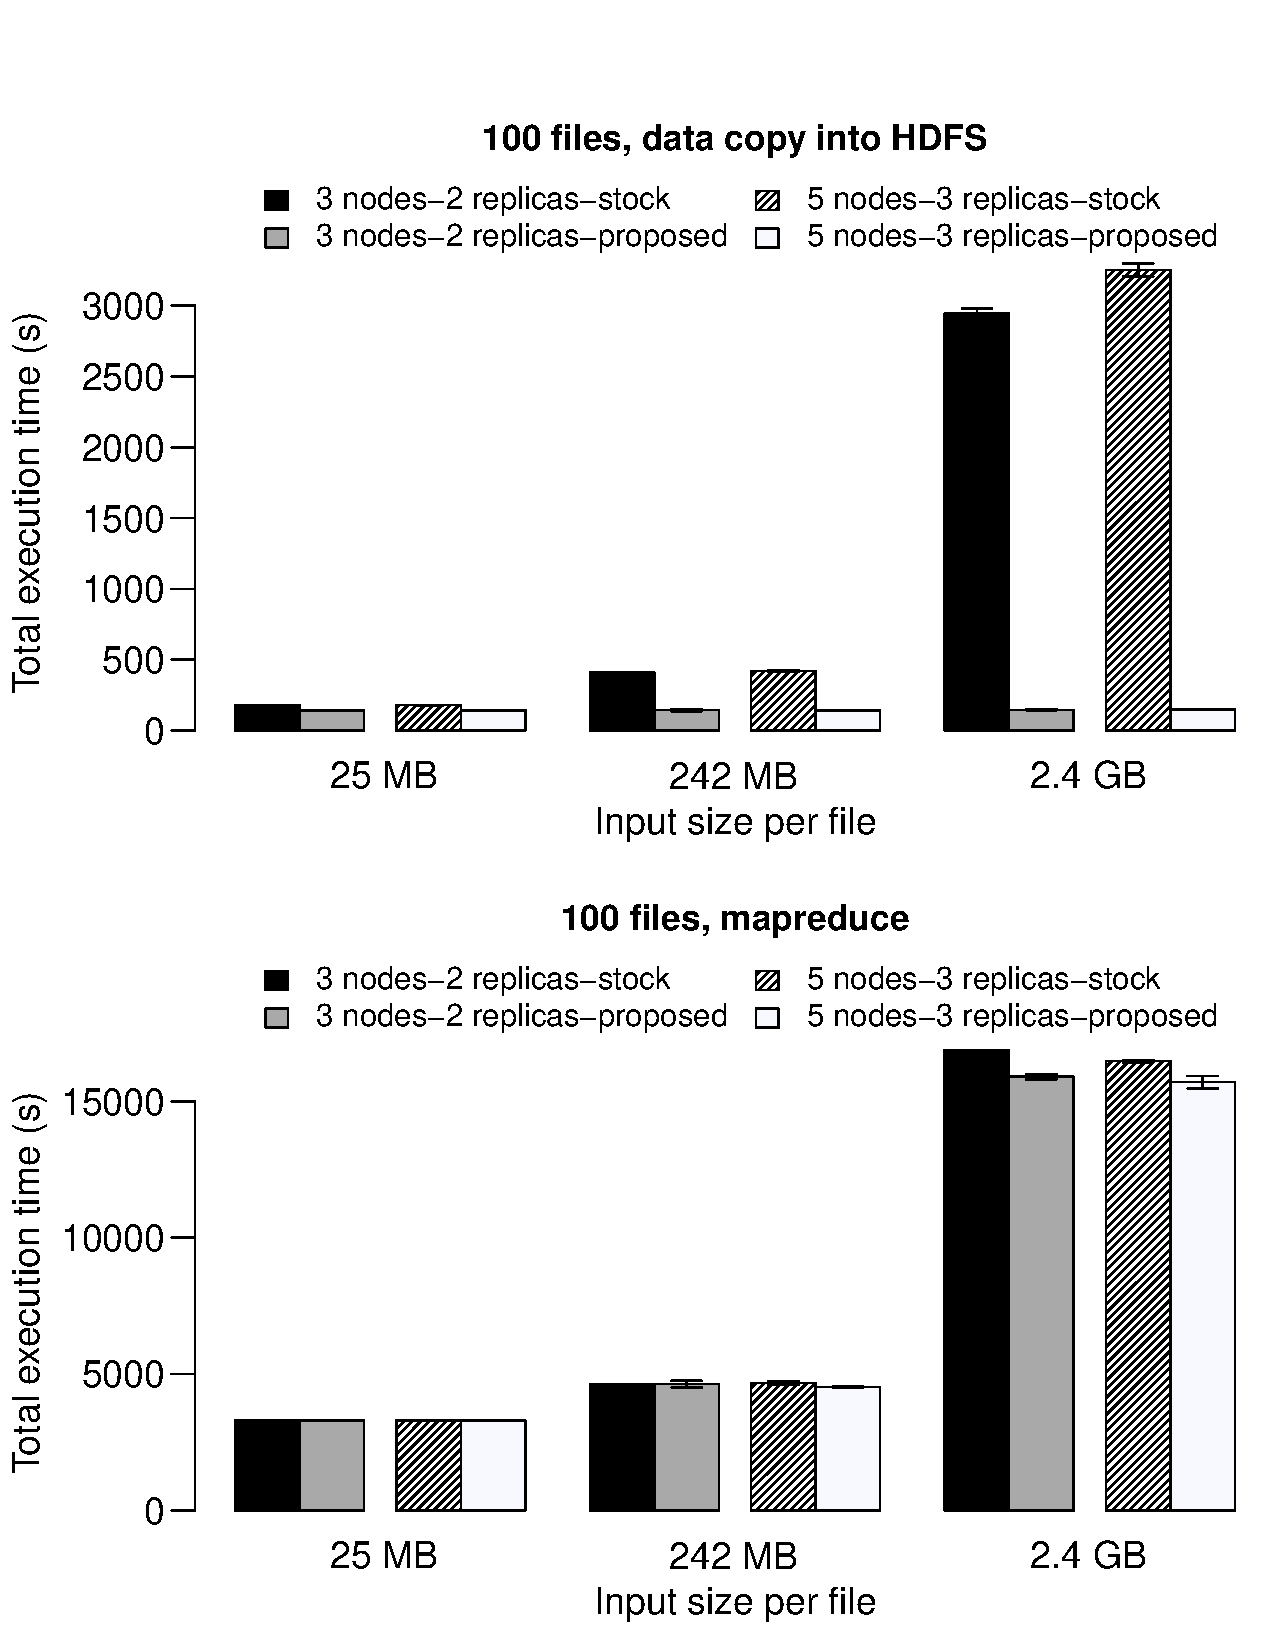
\includegraphics[width=\columnwidth, keepaspectratio]{result1.pdf}
\caption{Evaluation results for~\textit{Grep}}
\label{grepres}
\end{figure}

The upper sub-plot of Figure~\ref{grepres} shows the measurements of the total time it
takes to copy data into HDFS. As can be inferred, the proposed Hadoop implementation
takes significantly less time than stock Hadoop to copy data into HDFS; because, no
data is actually ingested into HDFS. As the input size per file is
increased from 25 MB to 2.4 GB, the time it takes to copy data into HDFS increases
for stock Hadoop. As no data is written to HDFS, that time stays constant
for the proposed implementation. An improvement of 95\% in terms of 
initial data copy performance is achieved and as the input size becomes larger, this improvement
will become even higher. Another conclusion from Figure~\ref{grepres} is that the
number of replicas or total storage nodes in the system does not have a significant
effect on the performance of the data copy phase.

Improving the performance of the MapReduce phase is not a primary goal of this work, as the
optimizations are targeted for the initial data copy phase; but, as the input size per file
becomes larger (i.e. 2.4 GB), nearly 5\% of improvement in MapReduce performance is observed
due to data-compute locality. This is achieved by using the object storage system to identify
replicas and force Hadoop to co-locate compute threads with the appropriate replica. Note that,
there are a variety of existing techniques to co-locate data and compute in Hadoop; but, they
do not help improving the performance of data copy phase, which is the primary goal of this work.
Similar to the data copy phase, the number of replicas or total storage nodes does not have a
significant effect on the performance of the MapReduce phase.

\subsubsection{Wordcount}
This section gives the evaluation results for the~\textit{Wordcount} benchmark.
~\textit{Wordcount} counts the number of occurrences of each word in a given file and
saves these numbers in an output file that is of similar size as the input.

Test parameters of the~\textit{Wordcount} benchmark are exactly the same
with those used for the~\textit{Grep} benchmark in Section~\ref{greptest};
except for the file sizes (29 MB, 286 MB or 2.8 GB per file).

\begin{figure}[!htbp]
\centering
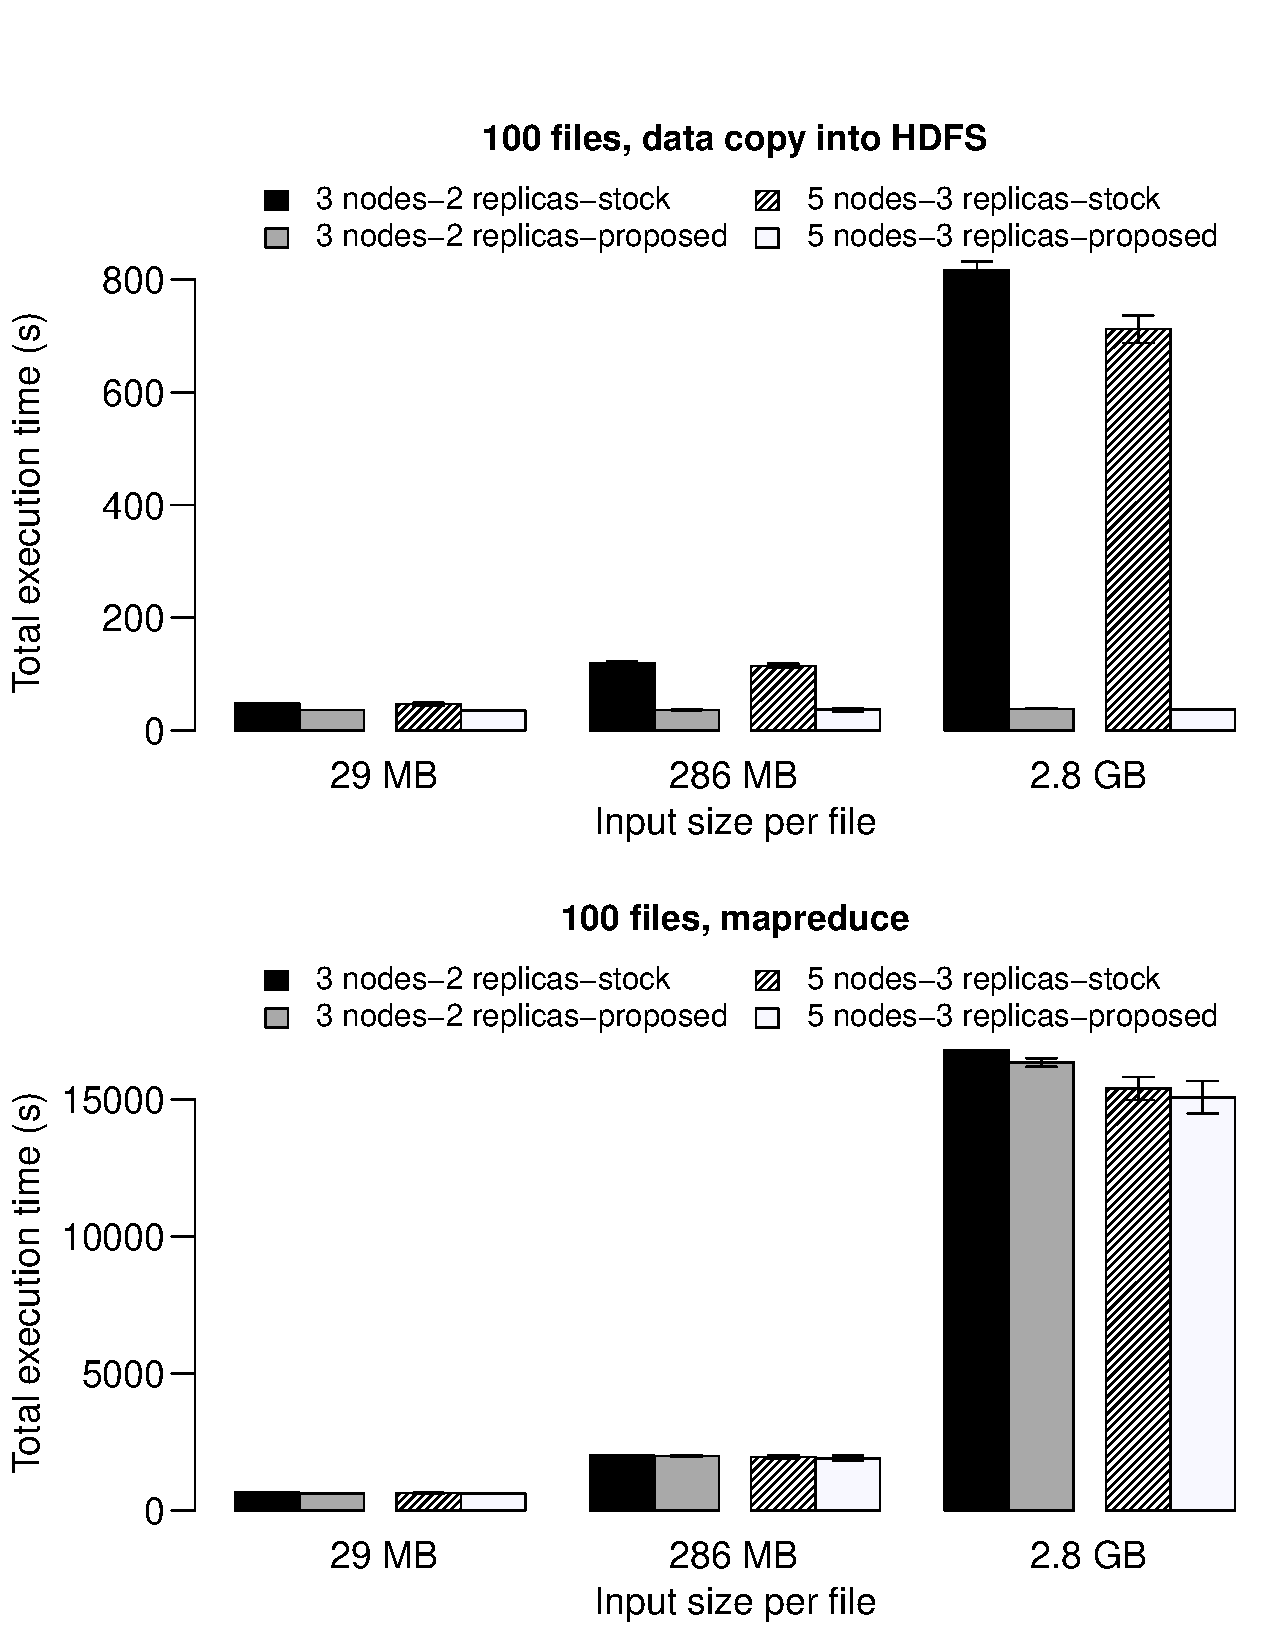
\includegraphics[width=\columnwidth, keepaspectratio]{result2.pdf}
\caption{Evaluation results for~\textit{Wordcount}}
\label{wordcountres}
\end{figure}


The upper sub-plot of Figure~\ref{wordcountres} shows the total time to copy data into HDFS.
The performance improvement is nearly 95\%, similar to the improvement observed for
the~\textit{Grep} benchmark in Section~\ref{greptest}. Additionally, increasing the
input size per file, the number of replicas or total storage nodes has similar impacts
and MapReduce performance is improved by nearly 5\% as data and computation are co-located,
with the number of replicas or storage nodes having no significant effect.

\subsubsection{TestDFSIO}
This section presents the experimental evaluation results for the~\textit{TestDFSIO}
benchmark. This benchmark generates its own input with its~\textit{write} option using
MapReduce, rather than the traditional data ingest method. It is possible to specify
the number and size of files to generate with~\textit{TestDFSIO} benchmark. In this test
case,~\textit{TestDFSIO} does not generate any input data, because its input already exists
in the system. When a~\textit{TestDFSIO} run is completed, it dumps statistics about the
benchmark performance (throughput, execution time, io rate etc.).

For the sake of simplicity and as the number of input files will not have a significant effect
on the outcome of~\textit{TestDFSIO} tests,~\textit{TestDFSIO} benchmark is tested with a single
file and the file size is varied between 500 MB and 50000 MB. Stock Hadoop creates these files with
the~\textit{write} option of~\textit{TestDFSIO} and then performs a read operation on them. The
implementation presented in this work performs a zero-length write that sets up symbolic links to
already existing data, followed by a read operation. These test steps are performed for both
3 nodes with 2 replicas and 5 nodes with 3 replicas.

\begin{figure}[!htbp]
\centering
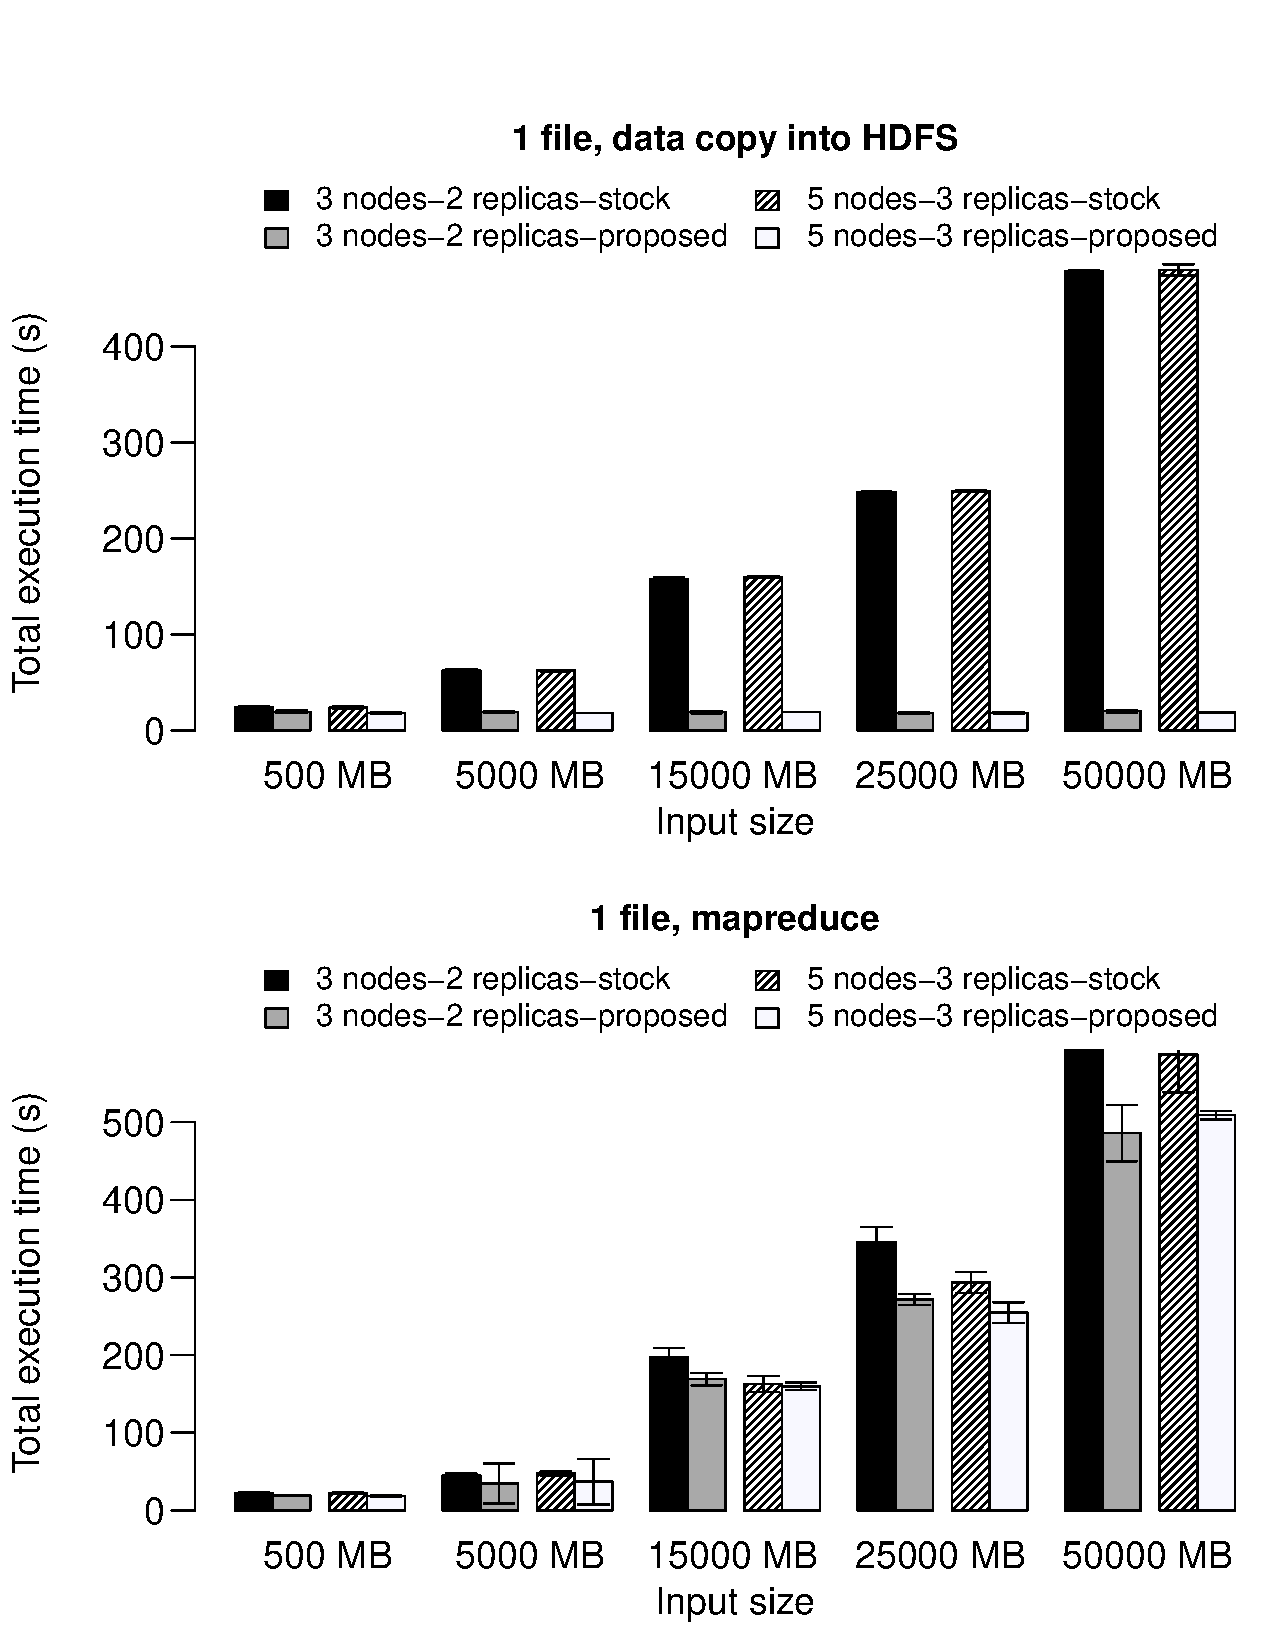
\includegraphics[width=\columnwidth, keepaspectratio]{result3.pdf}
\caption{Evaluation results for~\textit{TestDFSIO}}
\label{testdfsiores}
\end{figure}

Figure~\ref{testdfsiores} shows the data copy and MapReduce performance of the proposed implementation
compared with that of stock Hadoop. First conclusion to draw is that regardless of the input data size
and the number of replicas and storage nodes, our Hadoop implementation spends the same amount of time
for the initial ingestion of data. On the other hand, the time it takes for stock Hadoop to create the
data with the~\textit{write} option of~\textit{TestDFSIO} increases as the file size is increased
from 500 MB to 50000 MB. At 50000 MB, the proposed implementation achieves a 96\% improvement over the stock
Hadoop implementation in terms of data copy performance. For the MapReduce phase, as the file size
is increased, our Hadoop implementation performs better when compared to stock Hadoop.
Since local map tasks are used, which means data and computation are co-located, the time it takes
to shuffle mapper outputs to reducers is much smaller. Additionally,~\textit{TestDFSIO}
MapReduce phase is dominated by reading the generated data which happens totally local,
making the MapReduce improvement more apparent. As a result, MapReduce performance is improved
by nearly 20\% with the number of replicas or storage nodes having no significant effect.
~\textit{TestDFSIO} test results are highly variant and this is a known issue with
the~\textit{TestDFSIO} benchmark~\cite{hdfs941}.

\subsubsection{TeraSort}
Finally, this section presents the experimental evaluation results for the~\textit{TeraSort} benchmark.

Similar to the~\textit{TestDFSIO} benchmark,~\textit{TeraSort} generates its own input
with the~\textit{TeraGen} benchmark using MapReduce, rather than the traditional
data ingest method. The input data generated by~\textit{TeraSort} consists of 100-byte rows.
It is possible to specify the size of input data to be generated with~\textit{TeraGen}. While
evaluating the proposed changes,~\textit{TeraSort} does not generate any input data as its input
already exists.

The input size for~\textit{TeraSort} benchmark is varied between 5 GB, 10 GB and 50 GB during
the performance evaluations. Stock Hadoop implementation creates files of these sizes with the
~\textit{TeraGen} benchmark and then sorts them with~\textit{TeraSort}. Our Hadoop implementation performs
a zero-length write when~\textit{TeraGen} is executed and creates symbolic links to already existing data.
~\textit{TeraSort} sorts generated data and finally~\textit{TeraValidate} is executed to validate the
sorted data. This test case is performed for both 3 nodes with 2 replicas and 5 nodes with 3 replicas.

\begin{figure}[!htbp]
\centering
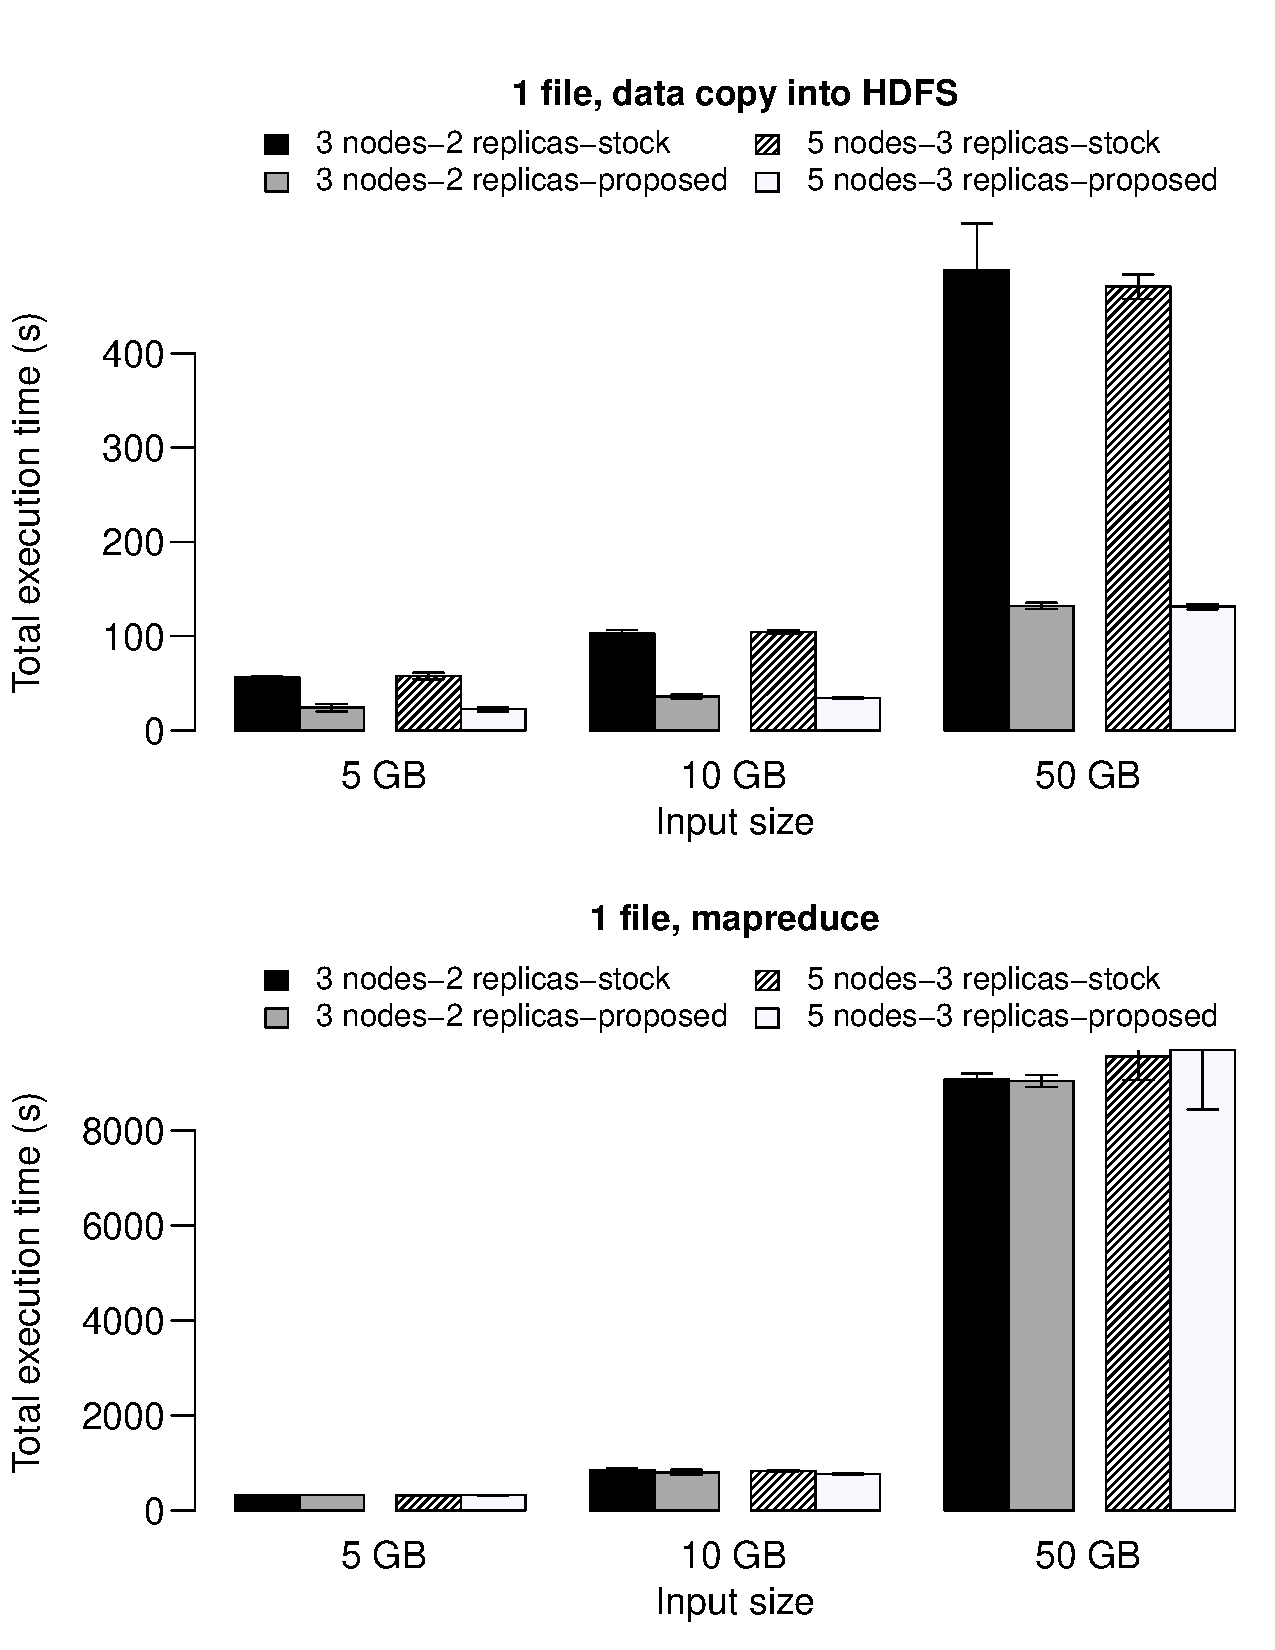
\includegraphics[width=\columnwidth, keepaspectratio]{result4.pdf}
\caption{Evaluation results for~\textit{TeraSort}}
\label{terasortres}
\end{figure}

The upper sub-plot of Figure~\ref{terasortres} shows that data copy times increase as the input
size is increased from 5 GB to 50 GB for both stock and proposed Hadoop. This is expected for stock
Hadoop; but, for our implementation, data copy times increase because records created by
the~\textit{TeraGen} are still processed one-by-one.~\textit{TeraGen} generates data in the format
of 100-byte records (i.e. to generate 6553600 bytes of data, 65536 records are needed) and it writes
data to each record individually. In the implementation presented in this work, these records
are created; but, actual data is not committed to HDFS resulting in empty records. As the input
size is increased from 5 GB to 50 GB, the number of records to create increases as well, which
in turn increases data copy time. Still, a data copy performance improvement by up to 73\% is
observed, which becomes even bigger with larger input sizes. Additionally, the number of replicas
and storage nodes does not affect the data copy performance significantly. For the MapReduce phase,
nearly 5\% improvement is observed due to data-compute locality, with the number of replicas or
storage nodes having no significant effect. MapReduce performance improvements in this
test case are not as high as those from~\textit{TestDFSIO}, as the MapReduce phase is not dominated by reads
only.
